\documentclass[11pt]{article}

\usepackage[english]{babel}
\usepackage[utf8]{inputenc}
\usepackage{amsmath}
\usepackage{amssymb}
\usepackage{graphicx}
\usepackage[colorinlistoftodos]{todonotes}
\usepackage{listings,multicol}
\usepackage{textcomp}
\usepackage{hyperref}
\usepackage{longtable}

\setlength{\oddsidemargin}{0.5cm} \setlength{\evensidemargin}{0cm}
\setlength{\textwidth}{16cm} \setlength{\textheight}{23cm}
\setlength{\topmargin}{-0.5cm}
\textheight 21.5cm


\begin{document}

\title{L4 NUMERICO UCSC}

\begin{minipage}{0.15\textwidth}

\includegraphics[width=\textwidth]{ucsc.png}
\end{minipage}
\begin{minipage}{0.9\textwidth}
{UNIVERSIDAD CAT\'OLICA}\\ 
{DE LA SANT\'ISIMA CONCEPCI\'ON}\\
{DEPARTAMENTO DE MATEM\'ATICA}\\ 
{ Y F\'ISICA APLICADAS}\\
\rule{0.66\textwidth}{.5pt} %Franco A. Milanese
\end{minipage}

\vspace*{0.5cm} \centerline {\bf\underline{Laboratorio 4, C\'alculo Num\'erico  IN1012C }}
\centerline{\textrm{Semana 19 de abril de 2015}}  \vspace{0.2cm}




% \textbf{Nombre:} \hspace{0.5\textwidth}\textbf{Carrera:}
% \vspace{0.1cm}
% \textbf{Profesor:}\hspace{0.5\textwidth} \textbf{ RUT:}
%  \begin{center}
%  \begin{tabular}{||p{2cm}|p{2cm}|p{2cm}||}
%  \hline
%  Pregunta 1 &  Pregunta 2 &     Total\\
%  \hline

%   \vspace{1.5cm} & &       \\
%  \hline
%  \end{tabular}
%  \end{center}
% Enviar documentos solicitados en el formato solicitado a \textbf{veranonumerico@gmail.com}.

\centerline{Introducci\'on  a MATLAB \circledR: gr\'aficas de funciones en tres dimensiones} 
%

\section{Gr\'aficas 3D}
MATLAB provee muchas opciones para visualizar datos 3D, inclusive trae incorporada 
la opci\'on de dibujar con colores, lo que permite poder visualizar una cuarta dimensi\'on. 
Entre las funcionalides incorporadas tiene dibujar curvas en el espacio, dibujar 
objetos definidos por alambres, superficies sombreadas, generar autom\'aticamente curvas de nivel, 
mostrar datos de volumen, especificar las fuentes de luz e inclusive mostrar im\'agenes. El comando 
\begin{verbatim}
 help graph3d
\end{verbatim}
retorna una lista de todas las funciones disponibles para hacer gr\'aficos 3D.

\section{\texttt{ez}-funciones}
Las librer\'ia de funciones \texttt{ez} contienen las siguientes para realizar gr\'aficos 3D.

\begin{enumerate}
 \item \texttt{ezplot3()}.
 
 Esta funci\'on permite graficar curvas param\'etricas en el espacio. Supongamos que 
 una curva param\'etrica en el espacio viene dada por las funciones $x(t)$, $y(t)$, $z(t)$ 
 \texttt{ezplot3()} por defecto asumir\'a que $t\in[0,2\pi]$. Ejemplo:

\begin{minipage}{0.4\textwidth}
      \begin{verbatim}
	x='t.*cos(3.*pi.*t)';
	y='t.*sin(3.*pi.*t)':
	z='t';
	ezplot3(x,y,z)
      \end{verbatim}
\end{minipage}
\begin{minipage}{0.5\textwidth}
      \begin{center}
      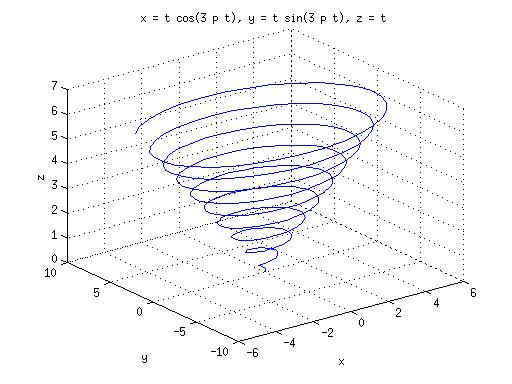
\includegraphics[width=\textwidth]{./ej1.jpg}
      \end{center}
\end{minipage}

\item \texttt{ezcountour()}

Las generaci\'on de curvas de nivel de curvas de nivel es sumamente sencilla 
con la funci\'on \texttt{ezcontour()}. Tan s\'olo especificamos la funci\'on 
de la forma $z=f(x,y)$ y podemos especificar el dominio de $x$ e $y$ deseado, por defecto 
$x,y\in [-2\pi,2\pi]$. Por ejemplo

\begin{minipage}{0.4\textwidth}
      \begin{verbatim}
	z='sin(x).*cos(y)./(x.^2+y^2+1)';
	ezcontour(z,[-3,3,-3,3]);
      \end{verbatim}
\end{minipage}
\begin{minipage}{0.5\textwidth}
      \begin{center}
      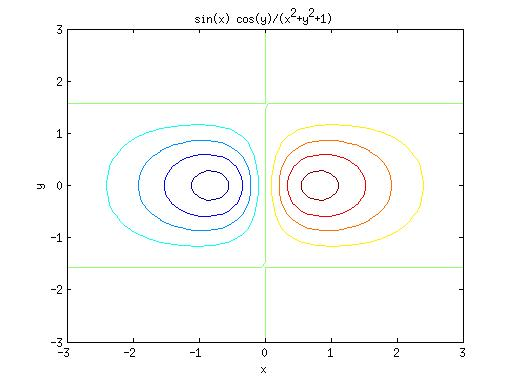
\includegraphics[width=\textwidth]{./ej2.jpg}
      \end{center}
\end{minipage}

\item \texttt{ezsurf()}

Para producir sorprendentes gr\'aficos 3D todo lo que necesitas es 
especificar la funci\'on a dibujar de la forma $z=f(x,y)$ y especificar 
el dominio para graficar. Por ejemplo

\begin{minipage}{0.4\textwidth}
      \begin{verbatim}
	z='sin(x).*cos(y)./(x.^2+y^2+1)';
	ezsurf(z,[-3,3,-3,3]);
      \end{verbatim}
\end{minipage}
\begin{minipage}{0.5\textwidth}
      \begin{center}
      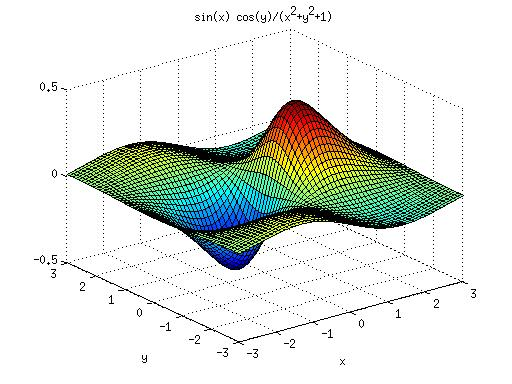
\includegraphics[width=\textwidth]{./ej3.jpg}
      \end{center}
\end{minipage}

\item \texttt{ezsurfc()}

Para combinar las curvas de nivel y gr\'afica de una superficie, utilizamos esta variante de
\texttt{ezsurf()}. Por ejemplo 

\begin{minipage}{0.4\textwidth}
      \begin{verbatim}
	z='cos(x.^2+y.^2)./(x.^2+y^2+1)';
	ezsurfc(z);
      \end{verbatim}
\end{minipage}
\begin{minipage}{0.5\textwidth}
      \begin{center}
      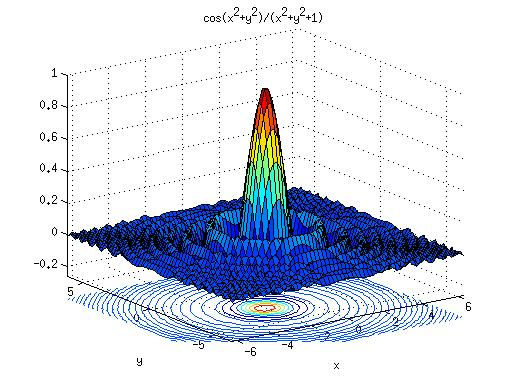
\includegraphics[width=\textwidth]{./ej4.jpg}
      \end{center}
\end{minipage}
\end{enumerate}

\section{Mallas y dibujos de superficies}
Las funciones para dibujar mallas y superficies sobre ellas son \texttt{mesh()} y \texttt{surf()}. 
Ente sus variaciones est\'an \texttt{meshc()}, \texttt{meshz()}, \texttt{surfc()} y \texttt{surfl()}. 
Todas estas funciones toman varios argumentos, las ejecuciones m\'as sencillas son de la forma 
\begin{verbatim}
 mesh(Z)
 surf(Z)
\end{verbatim}
donde \texttt{Z} representa una matriz. Usualmente las superficies son representadas por sus valores
en el eje $z$, evaluadas en una malla de pares $(x,y)$. En consecuencia, para crear el gr\'afico 
de una superficie necesitamos crear una malla de pares $(x,y)$ del dominio donde vamos a dibujar y encontrar 
la altura (coordenada $z$) de la superficie en cada punto de la malla. Observe que es lo mismo 
que hacemos para dibujar un gr\'afico de dos variables. MATLAB nos provee la funci\'on \texttt{meshgrid()} 
para crear una malla de puntos en un intervalo especificado.

\subsection{La funci\'on \texttt{meshgrid()}}

En MATLAB creamos dos matrices \texttt{X} e \texttt{Y} y escribimos las coordenadas $(x,y)$ 
de una malla como cada una de las componentes de estas matrices. Podemos evaluar la coordenada $z$ directamente 
en estas matrices.

Por ejemplo, si nos interesa mallar el dominio $[1,5]\times[1,5]$ con puntos equiespaciados 
de 1 unidad, podemos ejecutar
\begin{verbatim}
 x=1:5;
 [X,Y]=meshgrid(x,x);
\end{verbatim}
lo cual nos crea dos matrices \texttt{X} e \texttt{Y} cuyas componentes corresponder al malla representada en 
la figura \ref{fig:malla}. La valores de \texttt{X} e \texttt{Y} son

\begin{minipage}{0.4\textwidth}
 \begin{verbatim}
>> X

X =

     1     2     3     4     5
     1     2     3     4     5
     1     2     3     4     5
     1     2     3     4     5
     1     2     3     4     5

 \end{verbatim}
\end{minipage}  
\begin{minipage}{0.4\textwidth}
 \begin{verbatim}
  >> Y

Y =

     1     1     1     1     1
     2     2     2     2     2
     3     3     3     3     3
     4     4     4     4     4
     5     5     5     5     5

 \end{verbatim}
\end{minipage}
      \begin{figure}[htp]
      \begin{center}
      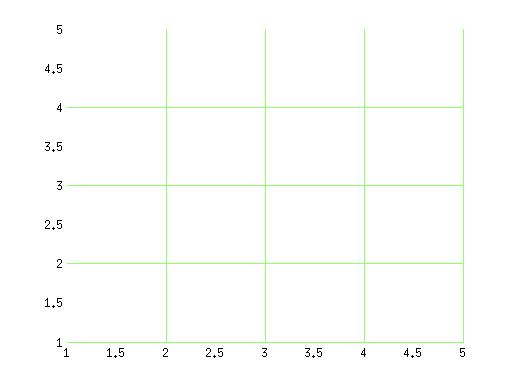
\includegraphics[width=0.6\textwidth]{./malla5.jpg}
      \caption{\sl Malla de $[0,5]\times[0,5]$ generado con \texttt{mesh(X,Y,zeros(5,5)}).}
      \label{fig:malla}
      \end{center}
      \end{figure}

 Para obtener las im\'agenes de una funci\'on en los puntos de esta malla solo resta operar componente a componente. Por 
 ejemplo, supongamos que nos interesa obtener las im\'agenes de la funci\'on $z=2*x+y-1$, en tal caso hacemos
 \begin{verbatim}
 Z=2.*X+Y-1;
 surf(X,Y,Z)
 \end{verbatim}
 y obtenemos lo representado en la figura \ref{fig:plano}
      \begin{figure}[htp]
      \begin{center}
      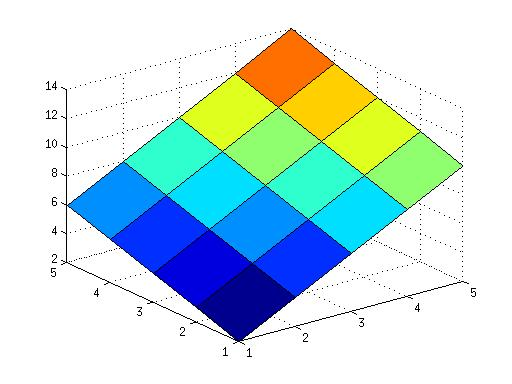
\includegraphics[width=0.6\textwidth]{./plano.jpg}
      \caption{\sl Secci\'on del plano de ecuaci\'on $2x+y-z-1=0$.}
      \label{fig:plano}
      \end{center}
      \end{figure} 

\newpage
\subsection{La funci\'on mesh()}
Baje y ejecute el rutero disponible en
\url{http://www.udec.cl/~fmilanese/codigo5.m }
este le permitir\'a generar los gr\'aficos
      \begin{center}
      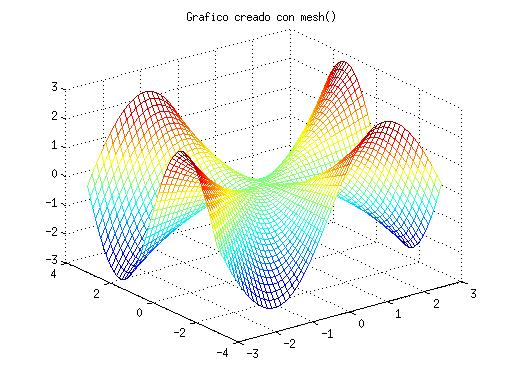
\includegraphics[width=0.4\textwidth]{./g1.jpg}
      \hspace{1cm}
      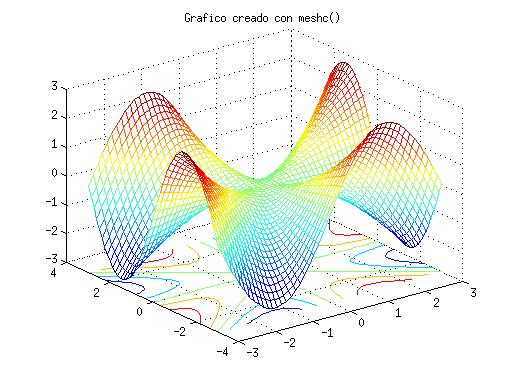
\includegraphics[width=0.4\textwidth]{./g2.jpg}
      \end{center}
      
\subsection{Algunos objetos en 3 dimensiones}

\texttt{sphere()}

El comando \texttt{sphere()} genera una esfera de radio uno 
centrada en el origen. Por ejemplo, puedes ejecutar 

\begin{minipage}{0.4\textwidth}
\begin{verbatim}
sphere(20)
axis('square')
\end{verbatim}
o
\begin{verbatim}
[x,y,z]=sphere(20);
surf(x,y,z)
axis('square')
\end{verbatim} 
\end{minipage}
\begin{minipage}{0.5\textwidth}
 \begin{center}
      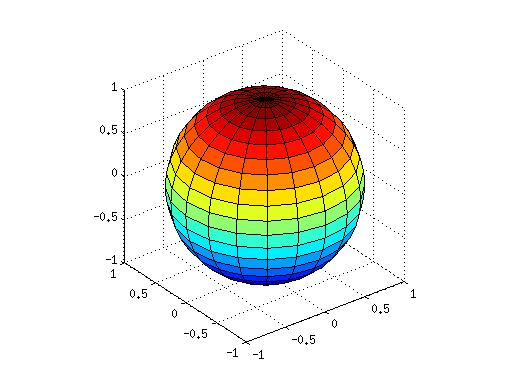
\includegraphics[width=\textwidth]{./esfera.jpg}
 \end{center}
\end{minipage}

\texttt{ellipsoid()}

El comando
\begin{verbatim}
 ellipsoid(cx,cy,cz,rx,ry,rz)
\end{verbatim}
genera un elipsoide de centro $(cx,cy,cz)\in\mathbb{R}^3$ y de semiejes $rx,ry,rz\in\mathbb{R}$. Por ejemplo


\begin{minipage}{0.4\textwidth}
\begin{verbatim}
cx = 0 ; cy = 0 ; cz = 0 ;
rx = 1 ; ry = 2 ; rz = .5 ;
ellipsoid(cx,cy,cz,rx,ry,rz)
axis('equal')
\end{verbatim} 
\end{minipage}
\begin{minipage}{0.5\textwidth}
 \begin{center}
      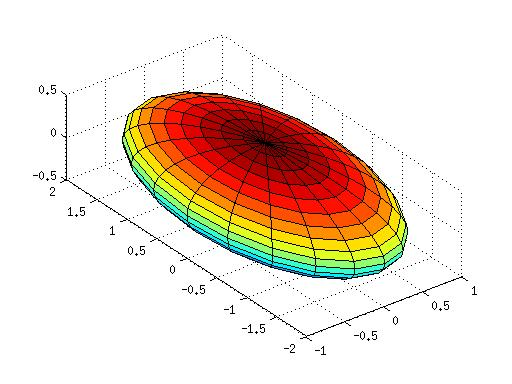
\includegraphics[width=\textwidth]{./elipsoide.jpg}
 \end{center}
\end{minipage}

\texttt{cylinder()}

Esta funci\'on de MATLAB grafica, o genera 
las matrices para graficar, un cilindro cuyo 
radio est\'a descrito como una funci\'on de la altura. Por ejemplo 

\begin{minipage}{0.4\textwidth}
\begin{verbatim}
z=[0:.02:1]';
r=sin(3 *pi*z)+2;
cylinder(r)
axis square
\end{verbatim} 
\end{minipage}
\begin{minipage}{0.5\textwidth}
 \begin{center}
      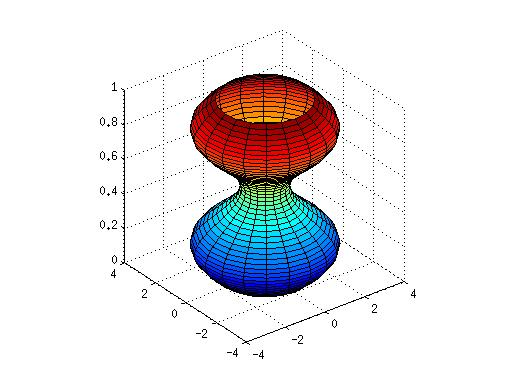
\includegraphics[width=\textwidth]{./cilindro.jpg}
 \end{center}
\end{minipage}



\section{Ejercicios}
\begin{enumerate}
 \item Grafique las siguientes funciones.
    \begin{multicols}{2}
    \begin{itemize}
     \item[a)]	$f(x,y)=x^2+y^2$,
     \item[b)]	$g(x,y)=\begin{cases}
               	          x+y & \text{ si } x>0\\
               	          x-y & \text{ si } x<0
               	         \end{cases}$,
    \item[c)]	$h(x,y)=g(f(x,y),y)$,
    \item[d)]	$x(t)=cos(\pi t), \, y(t)=sen(\pi t), \, z(t)=2t$ con $t\in[0,4]$, funci\'on dada param\'etricamente.
    \item[e)]	$r(x,y)=\frac{1}{x^2+y^2}$, obs: cuidado con dividir por cero.
    \end{itemize}
    \end{multicols}
    
 \item Utilize el comando \texttt{quiver()} o \texttt{quiver3()} para graficar los campos vectoriales
 \begin{multicols}{2}
    \begin{itemize}
     \item[a)] $
     \begin{array}{cll}
	f:\mathbb{R}^2 & \longrightarrow	& \mathbb{R}^2 \\
	(x,y)		& \longmapsto		& (x^2+y,-2x+y)	
     \end{array}
	   $
	   
       \item[b)] $
     \begin{array}{cll}
	g:\mathbb{R}^3 & \longrightarrow	& \mathbb{R}^3 \\
	(x,y,z)		& \longmapsto		& (cos(x),sin(y),3z)	
     \end{array}
	   $
    \end{itemize}
    \end{multicols}
    
 \item MATLAB permite realizar animaciones con uso de los comando \texttt{movie()}. La idea 
 principal es que si tienes una sucesi\'on de gr\'aficos que deseas animar, entonces 
 uses la funci\'on \texttt{movie()}, guardando cada gr\'afico como un cuadro de la animaci\'on como 
 parte de una gran matriz \texttt{M} y entonces animarlos con el comando \texttt{movie()}. Un gr\'afico 
 es almacenado usando el comando \texttt{getframe()}. Un ejemplo de como usar este c\'odigo se encuentra en
 \url{http://www.udec.cl/~fmilanese/animador.m}
 
 Utilice el c\'odigo anterior para generar una animaci\'on de las curvas
 
  \begin{itemize}
   \item[a)]  
 $
 f(x,n)=sin(x+n),x\in [0,1]
 $
 cuando el desfase $n\in\mathbb{R}$ varia entre $[0,2\pi]$.
 
  \item[b)]
  $
  f(x,y,n)=\frac{cos(x^2+y^2+n)}{x^2+y^2}
  $
  cuando el t\'ermino $n\in\mathbb{R}$ se hace variar entre $[0,10]$.
  \end{itemize}

 Procure que la animaci\'on muestre los cambios 
 de $n$ haciendo \texttt{title(num2str(n))} o lo que usted estime conveniente.
 
\item Haga un rutero que anime la deformaci\'on del ellipsoide
$\frac{x^2}{10^2} +y^2+z^2=2^2$ hasta transformarse en la esfera unitaria, suponga que 
primero se achica el semieje x y luego el radio.
 



\item Utilice el comando ellipsoid para graficar las superficies
\begin{eqnarray*}
\frac{x^{2}}{2}+\frac{y^{2}}{4}+\frac{z^{2}}{8}&=&1\\
\frac{(x-1)^{2}}{4}+\frac{(y+2)^{2}}{16}+\frac{z^{2}}{3^{2}}&=&1\\
\frac{x^{2}}{2}+\frac{y^{2}}{2}+\frac{z^{2}}{6}&=&x\\
\end{eqnarray*}

\item Cree un programa tipo \texttt{function} que grafique correctamente la esfera de radio $r$. Para ello utilice el comando \texttt{sphere()}.

\item Cree un programa tipo function que grafique tridimensionalmente el plano $ax+by+cz=k$, con $c\neq 0$. Agregue un mensaje de error si $c=0$. \textquestiondown Qu\'e pasa si $c=0$?

\item Cree un programa tipo function que grafique tridimensionalmente el plano $ax+by=k$, con $a,b\neq 0$. Agregue un mensaje de error si $a=0$ o $b=0$.

\item Cree un programa que grafique tridimensionalmente una recta.

% \item Descargue el archivo funn.m desde Ev@. Describa anal\'iticamente la funci\'on que describe y grafique las curvas de nivel en el eje XY y la superficie generada. Utilice la funci\'on planok para visualizar las curvas de nivel en los planos XZ e YZ.

\item Modifique el programa anterior para describir la funci\'on
$$
f(x,y)=\begin{cases}
	\frac{xy}{x-y} \text{ si } x\neq y\\
	1 				\text{ si } x=y
\end{cases}
$$
Grafique las curvas de nivel en el eje XY y la superficie generada.


\end{enumerate}


\end{document}  